\documentclass{beamer}

\usepackage{graphicx}
\usepackage{amsmath}
\usepackage{tikz}
\usetikzlibrary{arrows.meta,calc,shapes}

\usetheme{default}
\usefonttheme{serif}

\title{Introduction to the Finite Element Method}
\author{Laura A. Miller}
\date{\today}

\begin{document}

\begin{frame}
  \titlepage
  \begin{center}
    {\tiny AI tools were used to assist with formatting, organization, and clarification of the instructor's original notes.}
  \end{center}
\end{frame}

\begin{frame}{Resources}
  \begin{itemize}
    \item T. J. R. Hughes, \emph{The Finite Element Method: Linear Static and Dynamic Finite Element Analysis} (Dover, 2000).
    \item libMesh documentation: \url{https://libmesh.github.io}
    \item IBAMR: \url{https://ibamr.github.io}
    \item deal.II tutorial, step-3: \url{https://www.dealii.org/current/doxygen/deal.II/step_3.html}
  \end{itemize}
\end{frame}

\begin{frame}{What is the Finite Element Method?}
    \begin{itemize}
        \item The finite element method (FEM) is a numerical technique for solving complex engineering and mathematical problems.
        \item It's widely used in various fields, including structural analysis, fluid mechanics, heat transfer, and electromagnetics.
        \item FEM is particularly useful for problems with complex geometries, material properties, and boundary conditions.
    \end{itemize}
\end{frame}

\begin{frame}{Discretization}
    \begin{itemize}
        \item FEM divides a complex domain into smaller, simpler elements, such as triangles, quadrilaterals, or tetrahedra.
        \item This process is called discretization, and it transforms a continuous problem into a discrete one that can be solved numerically.
    \end{itemize}
    \begin{figure}
        \centering
        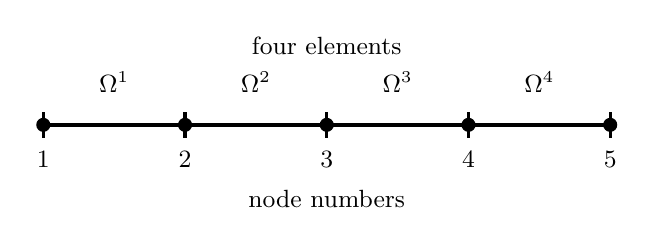
\begin{tikzpicture}[scale=0.9]
          \draw[very thick] (0,0) -- (8,0);
          \foreach \x in {0,2,4,6,8}{
            \draw[very thick] (\x,-0.18) -- (\x,0.18);
          }
          \foreach \x/\n in {0/1,2/2,4/3,6/4,8/5}{
            \filldraw (\x,0) circle (2.6pt);
            \node[below=6pt] at (\x,0) {\small $\n$};
          }
          \foreach \x/\e in {1/1,3/2,5/3,7/4}{
            \node[above=8pt] at (\x,0) {\small $\Omega^{\e}$};
          }
          \node[below=20pt] at (4,0) {\small node numbers};
          \node[above=22pt] at (4,0) {\small four elements};
        \end{tikzpicture}
        \caption{Example of domain discretization: a 1D domain split into four elements with five numbered nodes.}
    \end{figure}
\end{frame}

\begin{frame}{Shape Functions}
    \begin{itemize}
        \item Within each element, the solution is approximated using shape functions.
        \item Shape functions are simple functions defined over the element, typically polynomials.
        \item They interpolate the solution between the nodal values, which are the values of the unknown variables at the nodes of the element.
    \end{itemize}
    \begin{figure}
        \centering
        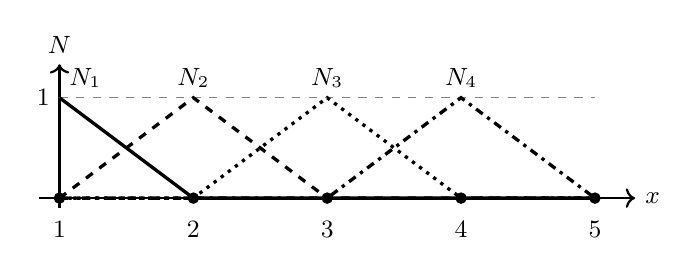
\begin{tikzpicture}[scale=0.85]
          \draw[->,thick] (-0.3,0) -- (8.6,0) node[right] {\small $x$};
          \draw[->,thick] (0,-0.15) -- (0,2.0) node[above] {\small $N$};
          \node[left] at (0,1.5) {\small $1$};
          \draw[dashed,gray] (0,1.5) -- (8,1.5);
          \foreach \x in {0,2,4,6,8}{
            \filldraw (\x,0) circle (2.2pt);
          }
          \foreach \x/\n in {0/1,2/2,4/3,6/4,8/5}{
            \node[below=5pt] at (\x,0) {\small $\n$};
          }
          \draw[very thick] (0,1.5) -- (2,0) -- (8,0);
          \draw[very thick,dashed] (0,0) -- (2,1.5) -- (4,0) -- (8,0);
          \draw[very thick,dotted] (0,0) -- (2,0) -- (4,1.5) -- (6,0) -- (8,0);
          \draw[very thick,dashdotted] (0,0) -- (4,0) -- (6,1.5) -- (8,0);
          \node[above right] at (0,1.5) {\small $N_1$};
          \node[above] at (2,1.5) {\small $N_2$};
          \node[above] at (4,1.5) {\small $N_3$};
          \node[above] at (6,1.5) {\small $N_4$};
        \end{tikzpicture}
        \caption{Piecewise-linear (hat) shape functions $N_1,\dots,N_4$ on the four-element mesh. Each equals 1 at its own node and 0 at every other node.}
    \end{figure}
\end{frame}

\begin{frame}{Shape Functions: A Mathematical Deep Dive}
    \begin{itemize}
        \item Shape functions are fundamental building blocks in the finite element method, used to approximate the solution within each element.
        \item They are typically chosen to be simple functions, such as polynomials, that are defined over the element domain.
        \item Shape functions are constructed to satisfy certain properties, such as:
        \begin{itemize}
            \item Interpolation: They must interpolate the solution at the nodal points, ensuring that the approximation matches the known values at these points.
            \item Continuity: They should exhibit a certain degree of continuity across element boundaries, depending on the order of the element and the requirements of the problem.
            \item Completeness: They should be able to represent constant and linear variations of the solution within the element, ensuring that the approximation can capture the essential behavior of the solution.
        \end{itemize}
    \end{itemize}
\end{frame}

\begin{frame}{Mathematical Representation of Shape Functions}
    \begin{itemize}
        \item Shape functions are typically represented using a local coordinate system ($\xi$, $\eta$) defined over the element domain.
        \item For example, in a 2D triangular element, the shape functions can be expressed as:
        \begin{align*}
        N_1(\xi, \eta) &= 1 - \xi - \eta \\
        N_2(\xi, \eta) &= \xi \\
        N_3(\xi, \eta) &= \eta
        \end{align*}
        where $N_1$, $N_2$, and $N_3$ are the shape functions associated with the three nodes of the triangle.
        \item These shape functions are linear polynomials that satisfy the interpolation, continuity, and completeness properties.
    \end{itemize}
\end{frame}

\begin{frame}{Properties of Shape Functions}
    \begin{itemize}
        \item Interpolation property: The shape function associated with a particular node has a value of 1 at that node and 0 at all other nodes.
        \item Partition of unity: The sum of all shape functions at any point within the element is equal to 1.
        \item Continuity: Lagrange shape functions are $C^0$ across element boundaries, meaning that they are continuous there but their derivatives generally are not; Hermite or spline elements are $C^1$ or higher.
        \item Completeness: The shape functions can represent constant and linear variations of the solution within the element.
    \end{itemize}
\end{frame}

\begin{frame}{Higher-Order Shape Functions}
    \begin{itemize}
        \item Higher-order shape functions, such as quadratic or cubic polynomials, can be used to achieve higher accuracy in the finite element approximation.
        \item These shape functions have more nodes per element and can capture more complex variations of the solution.
        \item However, they also increase the computational cost of the analysis.
    \end{itemize}
\end{frame}

\begin{frame}{Shape Functions in 3D}
    \begin{itemize}
        \item Shape functions can be extended to 3D elements, such as tetrahedra and hexahedra.
        \item The mathematical representation of 3D shape functions is more complex, but the fundamental principles remain the same.
    \end{itemize}
\end{frame}

\begin{frame}{Element Equations}
    \begin{itemize}
        \item The equations governing the behavior of each element are derived using variational principles or the Galerkin method.
        \item These equations relate the nodal values of the unknown variables to the element's properties and the external forces acting on it.
    \end{itemize}
\end{frame}

\begin{frame}{Element Equations in the Hybrid Immersed Boundary Finite Element Method}
    \begin{itemize}
        \item In the hybrid immersed boundary finite element method, the structure is discretized using finite elements, while the fluid is discretized using finite differences.
        \item This leads to a coupled system of equations that governs the behavior of the fluid-structure interaction.
        \item The element equations for the structure are derived from the principle of virtual work or the principle of minimum potential energy.
        \item These equations relate the nodal displacements and forces to the element stiffness matrix and the external forces acting on the element.
    \end{itemize}
\end{frame}

\begin{frame}{Mathematical Formulation of Element Equations}
    \begin{itemize}
        \item The element equations for a typical finite element can be expressed in matrix form as:
        \begin{equation*}
        \mathbf{K}^e \mathbf{u}^e = \mathbf{f}^e
        \end{equation*}
        (linear, small-strain case; hyperelastic IBFE structures give a nonlinear residual $\mathbf{r}(\mathbf{u}) = \mathbf{0}$ solved with a tangent stiffness)
        where:
        \begin{itemize}
            \item $\mathbf{K}^e$ is the element stiffness matrix
            \item $\mathbf{u}^e$ is the vector of nodal displacements for the element
            \item $\mathbf{f}^e$ is the vector of nodal forces for the element
        \end{itemize}
        \item The element stiffness matrix $\mathbf{K}^e$ depends on the material properties and geometry of the element.
        \item The nodal forces $\mathbf{f}^e$ include both external forces and forces due to the interaction with the fluid.
    \end{itemize}
\end{frame}

\begin{frame}{Assembly of Element Equations}
    \begin{itemize}
        \item The element equations are assembled into a global system of equations that governs the behavior of the entire structure.
        \item This assembly process involves combining the element stiffness matrices and nodal force vectors into global matrices and vectors.
        \item The resulting global system of equations can be expressed as:
        \begin{equation*}
        \mathbf{K} \mathbf{u} = \mathbf{f}
        \end{equation*}
        where:
        \begin{itemize}
            \item $\mathbf{K}$ is the global stiffness matrix
            \item $\mathbf{u}$ is the global vector of nodal displacements
            \item $\mathbf{f}$ is the global vector of nodal forces
        \end{itemize}
    \end{itemize}
\end{frame}

\begin{frame}{Coupling with Fluid Equations}
    \begin{itemize}
        \item The global system of equations for the structure is coupled with the fluid equations through the interaction forces.
        \item The interaction forces are calculated using the immersed boundary method, which involves spreading the forces from the Lagrangian structure to the Eulerian fluid grid and interpolating the fluid velocities back to the structure.
        \item The coupling between the structure and fluid equations leads to a nonlinear system of equations that must be solved iteratively.
    \end{itemize}
\end{frame}

\begin{frame}{Assembly and Solution}
    \begin{itemize}
        \item The element equations are assembled into a global system of equations that governs the behavior of the entire structure.
        \item This system of equations is then solved numerically to obtain the nodal values of the unknown variables.
    \end{itemize}
    \begin{figure}
        \centering
        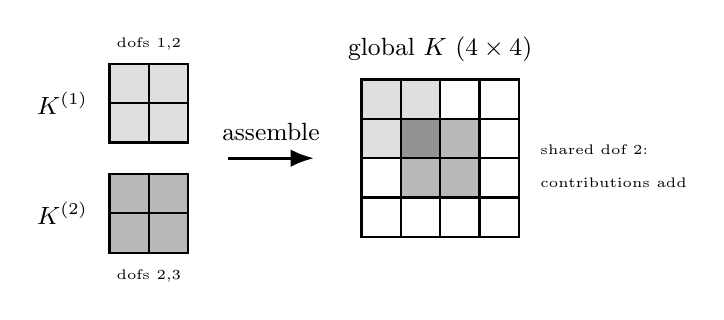
\begin{tikzpicture}[scale=1.0]
          % element matrix 1
          \begin{scope}[shift={(0,1.4)}]
            \fill[gray!25] (0,0) rectangle (1,1);
            \draw[step=0.5,thick] (0,0) grid (1,1);
            \draw[thick] (0,0) rectangle (1,1);
            \node[left] at (-0.15,0.5) {\small $K^{(1)}$};
            \node[above] at (0.5,1.05) {\tiny dofs 1,2};
          \end{scope}
          % element matrix 2
          \begin{scope}[shift={(0,0)}]
            \fill[gray!55] (0,0) rectangle (1,1);
            \draw[step=0.5,thick] (0,0) grid (1,1);
            \draw[thick] (0,0) rectangle (1,1);
            \node[left] at (-0.15,0.5) {\small $K^{(2)}$};
            \node[below] at (0.5,-0.1) {\tiny dofs 2,3};
          \end{scope}
          \draw[-{Latex[length=3mm]},very thick] (1.5,1.2) -- (2.6,1.2);
          \node[above] at (2.05,1.3) {\small assemble};
          % global matrix
          \begin{scope}[shift={(3.2,0.2)}]
            \fill[gray!25] (0,1) rectangle (1,2);      % element 1 block
            \fill[gray!55] (0.5,0.5) rectangle (1.5,1.5); % element 2 block
            \fill[gray!85] (0.5,1) rectangle (1,1.5);  % overlap
            \draw[step=0.5,thick] (0,0) grid (2,2);
            \draw[thick] (0,0) rectangle (2,2);
            \node[above] at (1,2.1) {\small global $K$ ($4\times 4$)};
            \node[right,align=left] at (2.15,0.9) {\tiny shared dof 2:\\ \tiny contributions add};
          \end{scope}
        \end{tikzpicture}
        \caption{Assembly: each element matrix is scattered into the rows and columns of its own degrees of freedom in the global matrix; entries for a shared node (dark square) receive contributions from both elements.}
    \end{figure}
\end{frame}

\begin{frame}{Types of Elements}
    \begin{itemize}
        \item FEM offers a variety of element types to model different problems, such as 1D, 2D, and 3D elements.
        \item The choice of element type depends on the geometry of the problem, the desired accuracy, and the computational cost.
    \end{itemize}
    \begin{figure}
        \centering
        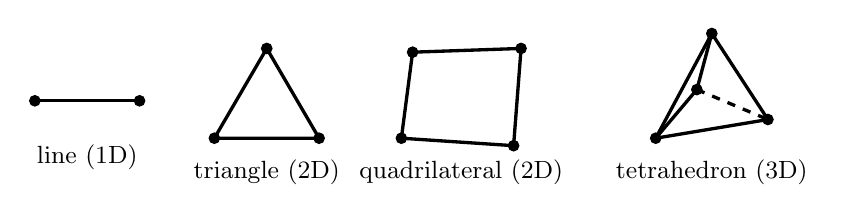
\begin{tikzpicture}[scale=0.95,every node/.style={font=\small}]
          % 1D line element
          \begin{scope}[shift={(0,0)}]
            \draw[very thick] (0,0.6) -- (1.4,0.6);
            \filldraw (0,0.6) circle (2pt);
            \filldraw (1.4,0.6) circle (2pt);
            \node at (0.7,-0.15) {line (1D)};
          \end{scope}
          % triangle
          \begin{scope}[shift={(2.4,0)}]
            \draw[very thick] (0,0.1) -- (1.4,0.1) -- (0.7,1.3) -- cycle;
            \filldraw (0,0.1) circle (2pt);
            \filldraw (1.4,0.1) circle (2pt);
            \filldraw (0.7,1.3) circle (2pt);
            \node at (0.7,-0.35) {triangle (2D)};
          \end{scope}
          % quadrilateral
          \begin{scope}[shift={(4.9,0)}]
            \draw[very thick] (0,0.1) -- (1.5,0.0) -- (1.6,1.3) -- (0.15,1.25) -- cycle;
            \filldraw (0,0.1) circle (2pt);
            \filldraw (1.5,0.0) circle (2pt);
            \filldraw (1.6,1.3) circle (2pt);
            \filldraw (0.15,1.25) circle (2pt);
            \node at (0.8,-0.35) {quadrilateral (2D)};
          \end{scope}
          % tetrahedron (wireframe)
          \begin{scope}[shift={(8.3,0)}]
            \coordinate (A) at (0,0.1);
            \coordinate (B) at (1.5,0.35);
            \coordinate (C) at (0.55,0.75);
            \coordinate (D) at (0.75,1.5);
            \draw[very thick] (A) -- (B) -- (D) -- cycle;
            \draw[very thick] (A) -- (C) -- (D);
            \draw[very thick,dashed] (C) -- (B);
            \filldraw (A) circle (2pt);
            \filldraw (B) circle (2pt);
            \filldraw (C) circle (2pt);
            \filldraw (D) circle (2pt);
            \node at (0.75,-0.35) {tetrahedron (3D)};
          \end{scope}
        \end{tikzpicture}
        \caption{Different types of finite elements: a 1D line element, 2D triangular and quadrilateral elements, and a 3D tetrahedron (shown as a wireframe).}
    \end{figure}
\end{frame}

\begin{frame}{Boundary Conditions}
    \begin{itemize}
        \item Boundary conditions are incorporated into the FEM model to represent the physical constraints of the problem.
        \item They can be essential boundary conditions (e.g., prescribed displacements) or natural boundary conditions (e.g., applied forces).
    \end{itemize}
\end{frame}

\begin{frame}{Applications of the Finite Element Method}
    \begin{itemize}
        \item FEM has numerous applications in various fields, including:
        \begin{itemize}
            \item Structural analysis (e.g., stress analysis of bridges, buildings, and aircraft)
            \item Fluid mechanics (e.g., simulation of blood flow, airflow over an airfoil)
            \item Heat transfer (e.g., thermal analysis of electronic components)
            \item Electromagnetics (e.g., design of antennas and waveguides)
        \end{itemize}
    \end{itemize}
\end{frame}

\begin{frame}{Conclusion}
    \begin{itemize}
        \item FEM is a powerful numerical technique for solving complex engineering and mathematical problems.
        \item It's widely used in various fields due to its versatility and ability to handle complex geometries, material properties, and boundary conditions.
        \item Understanding FEM is crucial for comprehending the hybrid immersed boundary finite element method, which combines the strengths of both FEM and the immersed boundary method to solve fluid-structure interaction problems.
    \end{itemize}
\end{frame}

\begin{frame}{Glossary (stress units, from the solids module)}
  \begin{description}
    \item[Stress] A measure of the force acting per unit area within a deformable body.
    \item[Tensor] A mathematical object that describes a multilinear relationship between sets of algebraic objects related to a vector space.
    \item[Cauchy Stress Tensor ($\boldsymbol{\sigma}$)] A second-order tensor that describes the state of stress at a point within a material.
    \item[Normal Stress] Stress acting perpendicular to a surface.
    \item[Shear Stress] Stress acting parallel to a surface.
    \item[Pascal (Pa)] The SI unit of pressure or stress, equal to one newton per square meter.
    \item[Pound per Square Inch (psi)] A unit of pressure or stress in the imperial and US customary systems.
    \item[Continuum Mechanics] The branch of mechanics that deals with the analysis of the kinematics and mechanical behavior of materials modeled as a continuous mass rather than as discrete particles.
  \end{description}
\end{frame}

\end{document}